%%% LaTeX Template
%%% This template is made for project reports
%%%	You may adjust it to your own needs/purposes
%%%
%%% Copyright: http://www.howtotex.com/
%%% Date: March 2011

%%% Preamble
\documentclass[paper=a4, fontsize=12pt]{scrartcl}
\usepackage[T1]{fontenc}
\usepackage{fourier}

\usepackage[utf8]{inputenc}
\usepackage[german]{babel}											
\usepackage[protrusion=true,expansion=true]{microtype}			
\usepackage{amsmath,amsfonts,amsthm}										
\usepackage[pdftex]{graphicx}													
\usepackage{url}
\usepackage{todonotes}


%%% Custom sectioning (sectsty package)
\usepackage{sectsty}												
\allsectionsfont{\centering \normalfont\scshape}	


%%% Custom headers/footers (fancyhdr package)
\usepackage{fancyhdr}
\pagestyle{fancyplain}
\fancyhead{}														% No page header
\fancyfoot[L]{\small Limiter auf dem XMOS DSP}		% You may remove/edit this line 
\fancyfoot[C]{}													% Empty
\fancyfoot[R]{\thepage}									% Pagenumbering
\renewcommand{\headrulewidth}{0pt}			% Remove header underlines
\renewcommand{\footrulewidth}{0pt}				% Remove footer underlines
\setlength{\headheight}{13.6pt}


%%% Equation and float numbering
\numberwithin{equation}{section}		% Equationnumbering: section.eq#
\numberwithin{figure}{section}			% Figurenumbering: section.fig#
\numberwithin{table}{section}				% Tablenumbering: section.tab#

\usepackage[
backend=biber,
style=alphabetic,
sorting=ynt
]{biblatex}
\addbibresource{dsp_refs.bib}

%%% Maketitle metadata
\newcommand{\horrule}[1]{\rule{\linewidth}{#1}} 	% Horizontal rule

\title{
		%\vspace{-1in} 	
		\usefont{OT1}{bch}{b}{n}
		\normalfont \normalsize \textsc{Jadehochschule Oldenburg} \\ [25pt]
		\horrule{0.5pt} \\[0.4cm]
		\huge Look-Ahead Limiter auf einem XMOS Board \\
		\horrule{2pt} \\[0.5cm]
}
\author{
		\normalfont 								\normalsize
        Stephanus Volke\\[-3pt]		\normalsize
        \today
}
\date{}


%%% Begin document
\begin{document}
\maketitle
\newpage
\section{Einleitung}
Folgender Bericht ist Ergebnis einer Projektarbeit, welche im Sommersemester 2015 an der Jadehochschule Oldenburg im Modul \textit{Digitale Signalprozessoren} unter Leitung von Dr. Uwe Simmer entstand. Inhaltlich beschäftigte sich diese mit der Weiterentwicklung eines im vorhergehenden Semester begonnen, ähnlichen Projektes, welches die Implementierung eines Audio Lookahead Limiters auf einem DSP. Aus diesem Grund soll in diesem Bericht nicht nochmals auf die theoretischen Grundlagen eines Limiters sowie Besonderheiten der Programmierung von digitalen Signalprozessoren in Festkommaarithmetik eingegangen werden. Für Informationen dazu sei auf den entsprechenden Bericht verwiesen \cite{VS15}.


\section{Projektvoraussetzungen}

Dieser Abschnitt befasst sich mit Rahmenbedingungen und Voraussetzungen, welche vor Beginn des Projektes gegeben waren, wobei in Soft- und Hardwaregegebenheiten unterschieden werden soll.

\subsection{Softwarevoraussetzungen}
Als Codebasis stand die in einem vorangegangenen Projekt, ebenfalls von Volke in Zusammenarbeit mit Schreiber erarbeitete Implementierung eines Limiteralgorithmus zur Verfügung \cite{CR00}. Grundlage desselbigen ist die bei Internetrecherche gefundene Realisierungsidee eines nicht weiter identifizierbaren Christians, welche die Besonderheit aufweist, die notwendige Gainregelung in der Attackphase komplett mittels FIR-Filter zu steuern. Das wiederum hat den großen Vorteil, dass der gewählte Schwellenwert wirklich punktgenau erreicht wird und das Ausgangssignal keinesfalls Samples enthält, welche diesen im Pegel überschreiten. Zur Veranschaulichung ist in Abbildung \ref{fig:old_limiter_bsb} der strukturelle Aufbau des Algorithmus dargestellt.

\begin{figure}[hbt]
  \centering
  \label{fig:old_limiter_bsb}
  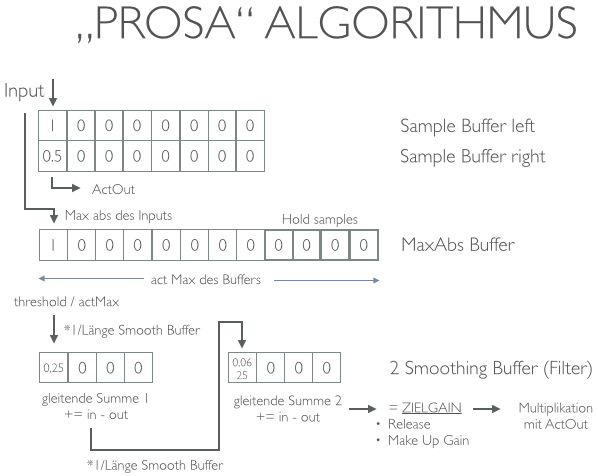
\includegraphics[width=0.8\textwidth]{graphics/prosalim_ablauf}
  \caption{Ablaufdiagramm des Lookahead Limiters vor der Erweiterung \cite{VS15}}
\end{figure}


Als frei wählbare Parameter stehen in der Implementierung von Volke und Schreiber der Threshold sowie die jeweiligen Zeiten für Attack- Hold- und Releasphase zur Verfügung. Die Umsetzung erfolge dabei so, dass der Limiter als \textit{loudness maximizer} arbeitet, also die Differenz zwischen Threshold und Vollaussteuerung automatisch mit dem limitierten Signal verrechnet, wodurch ein Ausgangssignal maximaler Lautstärke entsteht. 


\subsection{Hardwarevoraussetzungen}

\section{Vergleich der Hardwarearchitekturen}

\section{Erweiterungen des Codes}

\subsection{Dynamisierung}
\subsection{variable Releasezeit}
\subsubsection{Theoretische Grundlagen}
\subsubsection{Umsetzung}

\section{Evaluation}

\section{Fazit}




%%% End document

\printbibliography
\end{document}